The op amp in the circuit of Fig. \ref{fig:ee18btech11028_2_q} has an open-loop gain of $10^{5}$ and a single-pole rolloff with $\omega_{3dB}$ = 10 rad/s.  The circuit parameters are given in Table     \ref{table:ee18btech11028_2_parameters}

\begin{figure}[!ht]
	\begin{center}
		\resizebox{\columnwidth}{!}{\input{./figs/ee18btech11028/question_fig.tex}}
	\end{center}
\caption{}
\label{fig:ee18btech11028_2_q}
\end{figure}
%
\begin{table}[!ht]
    \centering
    \input{./tables/ee18btech11028/ee18btech11028_2_t1.tex}
    \caption{}
    \label{table:ee18btech11028_2_parameters}
\end{table}

\begin{enumerate}[label=(\alph*)]
\item Sketch a Bode plot for the loop gain.
\item  Find the frequency at which $ |GH|= 1$, and find the corresponding phase margin.
\item Find the closed-loop transfer function, including its zero
and poles. Sketch a pole-zero plot. Sketch the magnitude of
the transfer function versus frequency, and label the important parameters on your sketch.
\item  Find the unit step response of the system.
\end{enumerate}
\begin{enumerate}[label=\arabic*.,ref=\theenumi]
\numberwithin{equation}{enumi}
\item Find $G(s)$.
\\
\solution 
\begin{align}
    G(s) = \frac{10^5}{1 + \frac{s}{10}}
%    G(s) = \frac{10^5}{1 + \frac{s}{P_{11}}}
        \label{eq:ee18btech11028_2_2}
\end{align}


%\renewcommand{\thefigure}{\theenumi.\arabic{figure}}
%
\item Find $H(s)$ by drawing the equivalent circuit.
\\
\solution From Fig. \ref{fig:ee18btech11028_2_h}
%
\begin{align}
    H(s) &= \frac{V_{f}}{V_{o}}
    &= \frac{\frac{1}{sC_{f}}}{R_{f} + \frac{1}{sC_{f}}}
    &= \frac{1}{1 + \frac{s}{P_{21}}}
        \label{eq:ee18btech11028_2_1}
\end{align}
\begin{figure}[!ht]
	\begin{center}
		\resizebox{\columnwidth/2}{!}{\begin{circuitikz}
\ctikzset{bipoles/length=1cm}

\draw 
(0.5,1) node[ground]{}(0.5,1)--(1,1) to[C,l_=$C_{f}$,*-*]  (2,1)
(2.5,1)--(2.5,0.5)
(2,1)--(2.5,1)--(2.5,2)--(3,2) to[R=$R_{f}$] (4,2)--(4.5,2)--(4.5,1)

node at(2.5, 0.2){$V_{f}$}
node at(4.5, 0.7){$V_{o}$}
node at(2,1.3){$+$}
node at(1,1.3){$-$}
;
\end{circuitikz}
}
		
	\end{center}
\caption{Feedback loop}
\label{fig:ee18btech11028_2_h}
\end{figure}
%Also, feedback gain from Fig. \ref{fig:ee18btech11028_2_h},
\item Sketch a Bode plot for the loop gain.
\\
\solution
%Op-amp in our question has an open loop gain characterised by a single pole $P_{11} $ 
From Table \ref{table:ee18btech11028_2_parameters},
\begin{align}
    P_{21} = \frac{1}{R_{f}C_{f}} = 1000
\end{align}
The loop gain, 
\begin{align}
L(s) =  G(s)H(s) = \frac{10^5}{\brak{1+\frac{s}{10}}\brak{1 + \frac{s}{1000}}}
\end{align}
The amplitude and phase plots are available in Fig. \ref{fig:ee18btech11028_2_1} and Fig. \ref{fig:ee18btech11028_2_2} .

\renewcommand{\thefigure}{\theenumi.\arabic{figure}}
\begin{figure}[!ht]
    \centering
    \includegraphics[width=\columnwidth]{./figs/ee18btech11028/fig_1.eps}
    \caption{Magnitude plot}
    \label{fig:ee18btech11028_2_1}
\end{figure}


\begin{figure}[!ht]
    \centering
    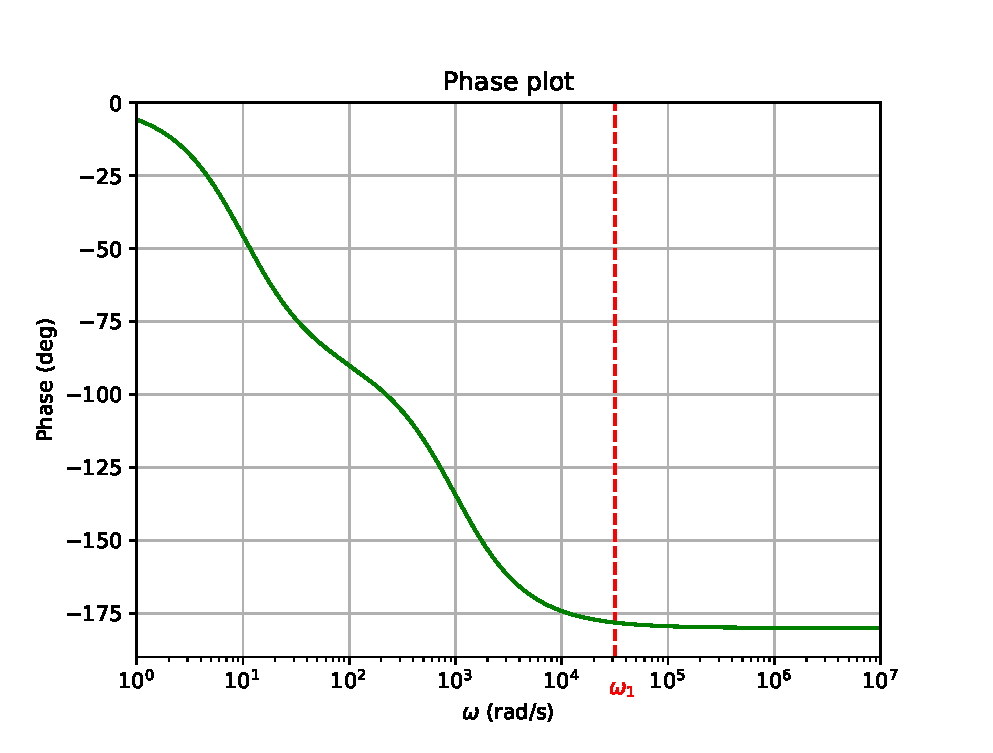
\includegraphics[width=\columnwidth]{./figs/ee18btech11028/fig_2.eps}
    \caption{Phase plot}
    \label{fig:ee18btech11028_2_2}
\end{figure}
\renewcommand{\thefigure}{\theenumi}
\item Find the frequency at which $ |GH|= 1$, and find the corresponding phase margin.
\\
\solution
Value of $\omega$ for unity magnitude can be obtained from Fig. \ref{fig:ee18btech11028_2_1} which is approximately $3 \times 10^{4}$.
More precise value can be obtained by solving for $\omega$ in,
\begin{align}
    \frac{10^{5}}{\sqrt{1 + \frac{w_{1}^{2}}{P_{1}^{2}}} \sqrt{1 + \frac{w_{1}^{2}}{P_{2}^{2}}}} = 1
\end{align}

Thus, 
\begin{align}
     \omega_{1} = 3.15 \times 10^{4} rad/s
\end{align}
The phase margin visibly from the Fig. \ref{fig:ee18btech11028_2_2} is very small.
\begin{align}
    PM &= 180 \degree - \tan^{-1}\brak{\frac{\omega_{1}}{10}} - \tan^{-1}\brak{\frac{\omega_{1}}{1000}}
      & = 1.84 \degree
\end{align}

\item Find the closed-loop transfer function, including its zero
and poles. Sketch a pole-zero plot. Sketch the magnitude of
the transfer function versus frequency, and label the important parameters on your sketch.
\\ 
\solution

\begin{align}
    T(s) = \frac{G(s)}{1 + G(s)H(s)}
    \\
\end{align}

From \eqref{eq:ee18btech11028_2_1} and \eqref{eq:ee18btech11028_2_2} we have,
\begin{align}
    \implies T(s) = \frac{10^{6}(s+1000)}{s^{2} + 1010s + 10^{4} + 10^{9}}
    \\
     \label{eq:ee18btech11028_2_3}
\end{align}

Zeros of closed loop transfer function,
\begin{align}
    Z_{1} = -1000
\end{align}

Similarly for poles,
\begin{align}
    s^{2} + 1010s + 10^{4} + 10^{9} = 0
    \\
    \implies P_{1}, P_{2} = -505 \pm j31618.9
\end{align}

\begin{figure}[!ht]
    \centering
    \includegraphics[width=\columnwidth]{./figs/ee18btech11028/fig_3.eps}
    \caption{Pole zero plot}
    \label{fig:ee18btech11028_2_3}
\end{figure}


\begin{figure}[!ht]
    \centering
    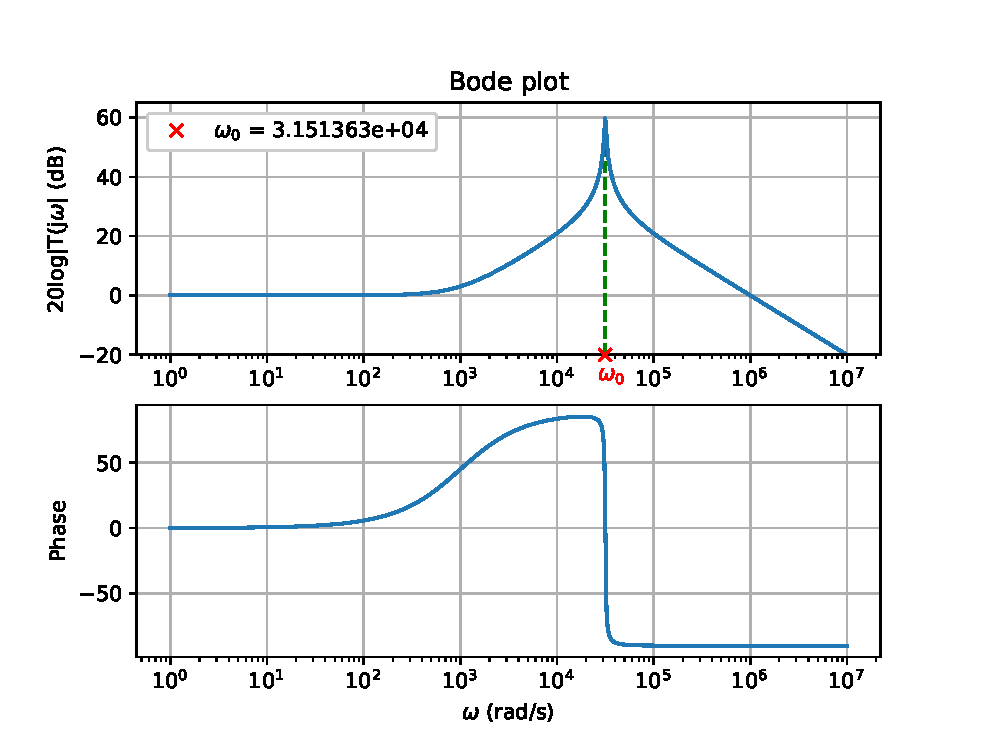
\includegraphics[width=\columnwidth]{./figs/ee18btech11028/fig_4.eps}
    \caption{Closed loop bode plot}
    \label{fig:ee18btech11028_2_4}
\end{figure}

Poles are at $\omega_{0} = 3.16 \times 10^{4}$

\item Closed loop unit step response.
\\
\solution 
\begin{figure}[!ht]
    \centering
    \includegraphics[width=\columnwidth]{./figs/ee18btech11028/step_response.eps}
    \caption{Unit step response}
    \label{fig:ee18btech11028_2_5}
\end{figure}


From \eqref{eq:ee18btech11028_2_3} Unit step response is,
\begin{align}
    Y_{\gamma}(s) = \frac{T(s)}{s}
\end{align}

We can calculate the steady state output voltage using Final value theorem,
\begin{align}
    \lim_{t\to\infty} V_{o}(t) = \lim_{s \to 0} sY_{\gamma}(s) \approx 1
\end{align}
which is analogous to plot in fig. \ref{fig:ee18btech11028_2_5}.
\item The following python code plots  Fig. \ref{fig:ee18btech11028_2_1}, Fig. \ref{fig:ee18btech11028_2_2}, Fig. \ref{fig:ee18btech11028_2_3}, Fig. \ref{fig:ee18btech11028_2_4} and Fig. \ref{fig:ee18btech11028_2_5}.
\begin{lstlisting}
codes/ee18btech11028/ee18btech11028_2.py
\end{lstlisting}
\item Simulate the circuit in Ngspice.
\\
\solution Following readme provides instructions about the simulation

\begin{lstlisting}
codes/ee18btech11028/spice/README.md
\end{lstlisting}

The following netlist simulates the closed loop unit step response for circuit in fig. \ref{fig:ee18btech11028_2_q}
\begin{lstlisting}
codes/ee18btech11028/spice/step_response.net
\end{lstlisting}
which is plotted using python code in,
\begin{lstlisting}
codes/ee18btech11028/spice/step.py
\end{lstlisting}
\begin{figure}[!ht]
    \centering
    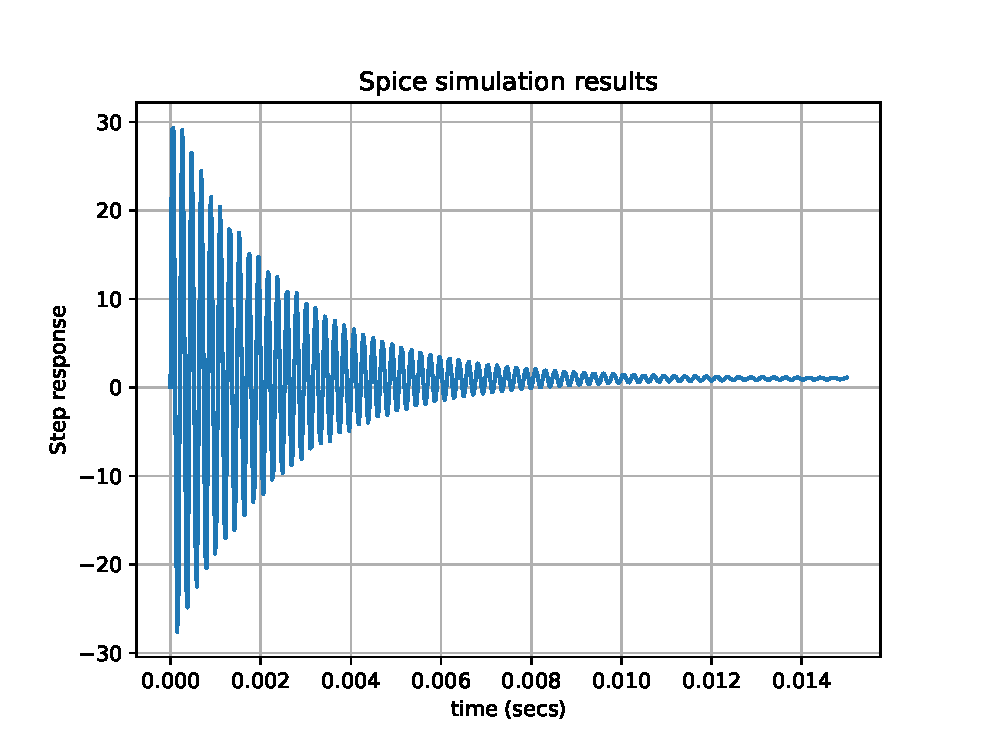
\includegraphics[width=\columnwidth]{./figs/ee18btech11028/spice_step_response.eps}
    \caption{spice simulation step response}
    \label{fig:ee18btech11028_2_6}
\end{figure}

As can be noticed in fig. \ref{fig:ee18btech11028_2_6} there is very minute difference in amplitude of the initial response of the circuit due to non-ideal nature of the circuit components. But rest of the response is identical including the steady state output voltage of 1.
\item
Circuit level schematic of op-amp used for simulation,
\begin{figure}[!ht]
	\begin{center}
		\resizebox{4\columnwidth/5}{!}{\begin{circuitikz}
\ctikzset{bipoles/length=1cm}

\draw 
(0,1)--(1,1)--(1,0.5) to [R = $ $] (1,-0.5)--(1,-1)--(0,-1)


(2, 0) to[I=$ $] (2,0) to (2,-1) %node[ground]{}
(2,0) -- (2,1)--(2.25,1) to[] (3,1) 
to [R = $ $] (3,-1) 
(3,1)--(4,1)to [C = $C_{p1}$](4,-1)
(2,-1) -- (2,-1)--(2.25,-1) to[] (5,-1)
(5,-1)--(5,1)--(5.25,1)--(5.75,1)to[R=$R_{out}$](6.75,1)

node at(0.5, 0){$R_{IN}$}
node at(3.5, -0.25){$R_{p1}$}
node at(0,1.25){$V_{+}$}
node at(0,-1.25){$V_{-}$}
node at(7.25,1){$V_{out}$}
node at(1.75,0.65){$G_{1}$}
node at(3,-1.5){$P_{1} $}
;
\end{circuitikz}
}
	\end{center}
\caption{}
\label{fig:ee18btech11028_2_7}
\end{figure}
is in fig. \ref{fig:ee18btech11028_2_7}
Since we need a single pole op-amp having $\omega_{3db}  =  10 rad/s$  $(f_{p1} = \frac{10}{2\pi} Hz)$,
we choose a $R_{p1}$ appropriately and calculate the value of $C_{p1}$ according to our single pole roll off frequency.
\begin{align}
    R_{p1}  = 1000 \ohm
    \\
    C_{p1} = \frac{1}{2  \pi f_{p1} R_{p1}}
\end{align}
The values corresponding to the components used for op-amp are given in table \ref{table:ee18btech11028_2_opamp_circuit}. 
\begin{table}[!ht]
    \centering
    \input{./tables/ee18btech11028/ee18btech11028_2_t2.tex}
    \caption{}
    \label{table:ee18btech11028_2_opamp_circuit}
\end{table}




\end{enumerate}
